\section{Closed-loop trajectory following for humanoid robots}
\label{closedloop}
%
%
This section proposes a control system for closed-loop trajectory
tracking while taking into consideration humanoid robots
specificities.
%
%
Closed-loop trajectory tracking consists in following a precomputed
trajectory while compensating for execution errors. Systems are often
composed of four components:
\begin{enumerate}
\item a trajectory generator component,
\item a localization component providing an estimation of the robot
  position,
\item an error estimation component computing the error between the
  planned position and the localization of the robot,
\item and a component reshaping the planned trajectory to compensate
  for the above error.
\end{enumerate}
%
%
The trajectory generator provides two reference data: the footstep
sequence, a set of footsteps $S_i$ such as \mbox{$0 \leq i \leq
  n^{\text{step}}$} and a whole-body trajectory \mbox{$\gamma(t \in
  [t_{\text{min}}, t_{\text{max}}]) \in \mathcal{C}$}. One advantage
of the proposed control scheme is to alter the future footstep
positions to avoid singularities. Given a known perturbation of the
footstep sequence, it is then possible to deduce the correction that
should be applied to the feet and center of mass trajectories. Once
those trajectories are computed, inverse geometry can be used to
regenerate the joints trajectories.
%
%
One iteration of the control loop is described by
Algorithm~\ref{fig:control_loop} and can be summarized as:
\begin{enumerate}
\item estimate the robot position,
\item compute the position error \mbox{$\delta \mathbf{x}$},
\item filter the error to avoid perturbing too much the initial
  trajectory and to absorb localization noise,
\item recompute the next steps positions to compensate execution
  errors and make sure the feet will land on the planned position,
\item check if the recomputed next step is feasible,
\item regenerate smooth trajectories for the feet, center of mass and
  ZMP.
\item regenerate the joints trajectories. This step is denoted by
  \mbox{$\gamma \bigoplus \delta \gamma$} in the algorithm. The
  \mbox{$\gamma \bigoplus \delta \gamma$} operation returns $\gamma$
  altered by the rigid transformation \mbox{$\delta \gamma$}. $\delta
  \gamma$ is the perturbation applied to the whole-body trajectory and
  is not directly computed as the inverse geometry is directly applied
  on the updated body positions.
\end{enumerate}
%
%
\begin{algorithm}
  \begin{algorithmic}
    \REQUIRE {$\gamma$, $t_{\text{current}}, t_{\text{next\_correction}}$}
    \ENSURE {$\gamma$, $t_{\text{current}}, t_{\text{next\_correction}}$}
    \IF {$\gamma(t_{\text{current}})$ is double support \AND
      $t_{\text{current}} \geq t_{\text{next\_correction}}$}
    \STATE estimate robot position $\mathbf{\hat{x}}$
    \STATE compute robot position error $\delta \mathbf{x}$
    \STATE compute offset $\delta \gamma$ absorbing the execution
    error $\delta \mathbf{x}$
    \IF {the perturbation $\delta \gamma$ can be applied}
    \STATE $\forall t \in [t_{\text{current}}, t_{\text{max}}],
    \gamma(t) \leftarrow \gamma(t) \bigoplus \delta \gamma(t)$
    \STATE $t_{\text{next\_correction}} \leftarrow t_{\text{current}} + 2 T_{\text{step}}$
    \ENDIF
    \ENDIF
    \STATE $\mathbf{q} \leftarrow \gamma(t_{\text{current}})$
    \STATE $t_{\text{current}} \leftarrow t_{\text{current}} + \Delta t$
  \end{algorithmic}
  \caption{Control loop at time $t_{\text{current}}$ achieving a
    closed-loop following of trajectory $\gamma$ (next correction will
    be applied at
    $t_{\text{next\_correction}}$). \label{fig:control_loop}}
\end{algorithm}
%
%
First, the robot position $\hat{\mathbf{x}}$ is perceived. The
localization system will not be detailed in this paper, see
\cite{08ijhr.stasse, 06humanoids.thompson} for instance for more
details. Although common limitations of these systems are taken into
account. The precision of the robot estimation does not decrease over
time, but can vary during the execution. This produces a noise which
may perturb the control scheme. The localization system can also fail
to provide an estimation or even sometimes provide aberrant values.
%
Secondly, an error $\mathbf{\delta \mathbf{x}}$ is computed by
comparing the planned and estimated position of the tracked reference
body. A threshold is applied to this value to bound the applied
corrections. In practice, it also filters out outliers and the noise
that the localization system may introduce in the system.
%
%
\begin{figure}[ht!]
  \begin{center}
    \begin{tikzpicture}[x=.40\textwidth,y=2.5cm]
      \def\w{0.3}
      \def\h{0.35}

      \def\ws{0.05}
      \def\hs{0.2}

      \def\noisex{0.01}
      \def\noisey{0.3}

      \foreach \dy in {0., 1.}
               {
                 \draw[pattern=dots,rounded corners]
                 (0.,0.25+\dy) rectangle (0.+\w,0.25+\dy+\h);

                 \draw[rotate=-10,rounded corners]
                 (\noisex,0.25+\noisey + \dy) rectangle
                 (\noisex+\w,0.25+\noisey+\dy+\h);

                 % left step planned
                 \filldraw[pattern=north east lines] (
                 0. + 0.1   * \w,
                 0.5 + \dy + 0.225 * \h)
                 rectangle (
                 0. + 0.1   * \w + \ws,
                 0.5 + \dy + 0.225 * \h + \hs);

                 % right step planned
                 \filldraw[pattern=north east lines] (
                 0. + 0.75 * \w,
                 \dy + 0.225  * \h)
                 rectangle (
                 0. + 0.75  * \w + \ws,
                 \dy + 0.225 * \h + \hs);

                 % left step real
                 \draw[rotate=-10] (
                 \noisex + 0.1   * \w,
                 0.5 + \noisey + \dy + 0.225 * \h)
                 rectangle (
                 \noisex + 0.1   * \w + \ws,
                 0.5 + \noisey + \dy + 0.225 * \h + \hs);

                 % right step real
                 \draw[rotate=-10] (
                 \noisex + 0.75 * \w,
                 \noisey + \dy + 0.225  * \h)
                 rectangle (
                 \noisex + 0.75  * \w + \ws,
                 \noisey + \dy + 0.225 * \h + \hs);
               }

               \draw[smooth,-,thick]
               (0.75 * \w + \ws/2.,\h/2.) --
               (0.75 * \w + \ws/2.,1.+\h/2.)
               node[midway,left]
               {
                 $\gamma$
               };

               \draw[smooth,rounded corners=1ex,-,thick]
               (0.75 * \w + \ws/2. + 0.03,0.15+\h/2. + 0.15) --
               (0.75 * \w + \ws/2. + 0.03 + 0.03,0.15+\h/2. + 0.15 + 0.4) --
               (0.75 * \w + \ws/2.,1.+\h/2.)
               node[at start,right]
               {
                 $\gamma \bigoplus \delta \gamma$
               };

               \draw[smooth,rounded corners=1ex,<->,thick]
               (-0.02, 0.25+0.45) --
               (-0.03, 0.25+0.35) --
               (-0.02, 0.25+0.25)
               node[at start,left]
               {
                 $\Delta r_z$
               };

               \draw[smooth,rounded corners=1ex,<->,thick]
               (-0.02, 0.25+0.) --
               (-0.02, 0.25+0.15)
               node[midway,left]
               {
                 $\Delta x$
               };

               \draw[smooth,rounded corners=1ex,<->,thick]
               (0., 0.25-0.1) --
               (0.03, 0.25-0.1)
               node[midway,below]
               {
                 $\Delta y$
               };

               \path node (txt1) at (0.075+\w,0.25+0.)
                     [shape=rectangle,draw,color=white]
                     {\color{black} $\mathbf{x}$};

               \path node (txt1) at (0.08+\w,0.25+0.3)
                     [shape=rectangle,draw,color=white]
                     {\color{black} $\mathbf{\hat{x}}$};

    \end{tikzpicture}
  \end{center}
  \caption{Correction of the next step due to a position error. Dotted
    rectangles are the planned positions $\mathbf{x}$ of the robot
    waist and feet before and after the next step. Non-dotted
    rectangles corresponds to the robot localization
    $\mathbf{\hat{x}}$. Error w.r.t to axis X, Y and yaw rotation is
    \mbox{$(\Delta x, \Delta y, \Delta r_z) = \delta \mathbf{x}$,
      $\gamma$} the reference trajectory and $\delta \gamma$ the
    corrected trajectory reaching the planned
    step. \label{fig:footstepreplan}}
\end{figure}
%
%
%
Then, the relative position of the next footstep w.r.t. to the current
one is changed to compensate the perceived
error. Fig.~\ref{fig:footstepreplan} illustrates this process.
%
%
From this point, smooth trajectories can be regenerated for feet and
center of mass. To ensure smoothness, the trajectory correction is
progressively applied during the next two steps. To finish, joint
values are recomputed using these new reference trajectories.
%
%
%
Additionally, a test is added to check that a correction can be
computed for the current time $t_{\text{current}}$. A correction can
be applied if no correction is being applied,
i.e.\ \mbox{$t_{\text{current}} \geq t_{\text{next\_correction}}$} and if the
robot is in the double support phase. Indeed starting a correction in
the middle of a step would be dangerous and starting a correction
while another correction is being applied would lead to erroneous
results.
%
%
Previous works such as \cite{04humanoids.harada, 07icra.morisawa} aim
at allowing sudden changes in the robot trajectory. The proposed
control scheme is different and aim at following as closely as
possible a preplanned trajectory.
%
%
%\vspace{0.3cm}
\paragraph{Estimation of the position error}
%
We make the assumption that an external system provides
\mbox{$\hat{\mathbf{x}} \in \text{SE}(2)$}, an estimation of the
current robot position.
%
If $\mathbf{x} \in \text{SE}(2)$ is the robot planned position and
$\hat{\mathbf{x}} \in \text{SE}(2)$ the robot localization, the
position error is defined by: $\mathbf{\delta x} = \mathbf{x} . \hat{\mathbf{x}}^{-1}$\label{eq:errorpos}
%
%\begin{equation} \label{eq:errorpos}
%  \mathbf{\delta x} = \mathbf{x} . \hat{\mathbf{x}}^{-1}
%\end{equation}
%
%In Eq. (\ref{eq:errorpos}), $\mathbf{\delta x}(t)$ can be
In the previous equation, $\mathbf{\delta x}(t)$ can be
interpreted as the planned robot position with respect to the current
robot position at time $t$. By consequence, at the beginning of the
trajectory $t_{\text{min}}$, the error is always equal to zero: $\delta \mathbf{x}(t_{\text{min}}) = 0$ \label{eq:errorpos_prop}
%
%\begin{equation} \label{eq:errorpos_prop}
%  \delta \mathbf{x}(t_{\text{min}}) = 0
%\end{equation}
%
%\vspace{0.3cm}
\paragraph{Footstep sequence modification}
%
%
Given a position error of the waist, it is possible to alter the
remaining steps in the footstep sequence to absorb this offset.
%
The purpose of this step is to take into consideration that the
previous step has not been executed correctly, leading to a different
relative position than the one which has been initially planned. To
cancel the error, the next footsteps positions will be modified
so that the robot will step in the planned locations.
%
%
The footstep positions are \mbox{$S \in
  \text{SE}(2)^{n^\text{step}}$}. Let consider $\mathbf{\delta {x}}$,
the current position error, \mbox{$S^{\text{future}} \subset S$} the
steps which have not been played yet. The footstep positions will be
changed according to the following computation: $\forall s \in S^{\text{future}}, s \gets \mathbf{\delta {x}} . s$ \label{eq:footstepmodif}
%
%\begin{equation} \label{eq:footstepmodif}
%  \forall s \in S^{\text{future}}, s \gets \mathbf{\delta {x}} . s
%\end{equation}
%
%
%\vspace{0.3cm}
\paragraph{Whole-body trajectories modification}
%
A new placement of the next feet has been computed. It is now necessary
to modify the two feet and the center of mass trajectories
synchronously to reach the corrected foot prints.
%
The correction is computed by considering the simplified model
introduced in section \ref{problem}. Hence, no hypothesis is done on
the strategy used to plan the reference trajectories. One interest of
this approach is to totally dissociate the planning and correction
algorithms. To compute a small perturbation the simplified model is
sufficient. It allows extremely reactive correction without
compromising the overall trajectory quality.
%
%
The linearized inverse pendulum model allows the computation of the
center of mass trajectory $\mathbf{c}(t)$ given a ZMP trajectory
$\mathbf{z}(t)$ by solving Eq.~(\ref{eq:zmp1}). Considering $\mathbf{r}$ a
polynomial depending only of $\mathbf{z}$, $(V_x, V_y, W_x, W_y)$ free
parameters used to constrain the initial position and velocity of the
center of mass, a general following form of a polynomial center of
mass trajectory is:
%
\begin{equation} \label{eq:zmpsol}
  \mathbf{c}(t) = \cosh(\sqrt{\frac{g}{z_c}}.t) . \mathbf{V} + \sinh(\sqrt{\frac{g}{z_c}}.t) . \mathbf{W} + \mathbf{r}(t)
\end{equation}
%
Given the formulation in Eq.~(\ref{eq:zmpsol}), it is possible to
continuously modify the center of mass trajectory to make it follow
\mbox{$\bar{\mathbf{z}}(t)$} the corrected trajectory. This new
trajectory can be expressed as the sum of two polynomials:
%
\begin{equation} \label{eq:zmpsolcor}
  \bar{\mathbf{c}}(t) = \cosh(\sqrt{\frac{g}{z_c}}.t) . \mathbf{V} +
  \sinh(\sqrt{\frac{g}{z_c}}.t) . \mathbf{W} + \mathbf{r}(t) + \mathbf{\Delta}(t)
\end{equation}
%
To apply smoothly the correction from $t_1$ to $t_2$, several
constraints expressed in Eq.~\ref{eq:cst} have to be respected.
$\delta \mathbf{x}_x$ and $\delta \mathbf{x}_y$ are respectively the
$x$ and $y$ components of the 2d rigid transformation $\delta
\mathbf{x}$.
%
\begin{equation}
\begin{aligned}
  \mathbf{\Delta}(t_1) &= \frac{\partial \mathbf{\Delta}}{\partial t}(t_1) = \frac{\partial
    \mathbf{\Delta}}{\partial t}(t_2) = 0\\
  \mathbf{\Delta}(t_2) &= \left(
  \begin{array}{c}
    \delta \mathbf{x}_x \\
    \delta \mathbf{x}_y
  \end{array}
  \right)
\end{aligned}
\label{eq:cst}
\end{equation}
%
\begin{figure}[ht!]
  \begin{center}

    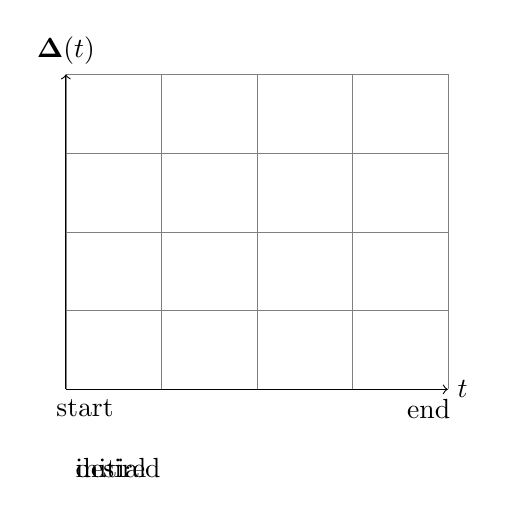
\begin{tikzpicture}[x=.40\textwidth,y=2.cm]%FIXME 2.5
      \def\xmin{0.}
      \def\xmax{1.}
      \def\ymin{0.5}
      \def\ymax{2.5}

      % grid
      \draw[style=help lines, ystep=.5, xstep=.25] (\xmin,\ymin) grid
      (\xmax,\ymax);

      % axes
      \draw[->] (\xmin,\ymin) -- (\xmax,\ymin) node[right] {$t$};
      \draw[->] (\xmin,\ymin) -- (\xmin,\ymax) node[above]
           {$\mathbf{\Delta}(t)$};

      % xticks and yticks
      \node at (0.05, \ymin) [below] {start};
      \node at (0.95, \ymin) [below] {end};

      \draw[color=black, domain=\xmin:\xmax] plot[id=cur]
      function{1} node [right] {initial};

      \draw[color=black, domain=\xmin:\xmax] plot[id=des]
      function{2} node [right] {desired};

      \draw[color=black, domain=\xmin:\xmax] plot[id=trans]
      function{-2. * x * x * x + 3 * x * x + 1} node [below] {};

    \end{tikzpicture}
  \end{center}
  \caption{Polynomial curve $\mathbf{\Delta}(t)$ providing a smooth
    transition between feet and center of mass
    trajectories. \label{fig:transition}}
\end{figure}
%
These four constraints determine the polynomial four parameters
leading to the curve illustrated by Fig.~\ref{fig:transition}.
%
%
\begin{figure}[ht!]
  \begin{center}
    \begin{tikzpicture}
      \begin{axis}[
          xlabel=time ($\mathrm{s}$),
          ylabel=$x$ position ($\mathrm{m}$),
          no markers
          ]

        \addplot[
          red,
          dashed
        ] table[
          x expr=(\thisrowno{0}-0)*0.005
        ] {dat/feet_follower_feet-follower-com.dat};
        \label{comcorr}
        \addplot[
          red,
        ] table[
          x expr=(\thisrowno{0}-0)*0.005,
          y expr=\thisrowno{1}-0.
        ] {dat/feet_follower_correction-com.dat};
        \label{com}

        \addplot[
          blue,
          dashed
        ] table[
          x index=0,
          y index=4,
          x expr=(\thisrowno{0}-0)*0.005
        ] {dat/feet_follower_feet-follower-left-ankle.dat};
        \label{lfcorr}

        \addplot[
          blue
        ] table[
          x index=0,
          y index=4,
          x expr=(\thisrowno{0}-0)*0.005,
          y expr=\thisrowno{4}-0.
        ] {dat/feet_follower_correction-left-ankle.dat};
        \label{lf}

        \addplot[
          green,
          dashed
        ] table[
          x index=0,
          y index=4,
          x expr=(\thisrowno{0}-0)*0.005
        ] {dat/feet_follower_feet-follower-right-ankle.dat};
        \label{rfcorr}

        \addplot[
          green
        ] table[
          x index=0,
          y index=4,
          x expr=(\thisrowno{0}-0)*0.005,
          y expr=\thisrowno{4}-0.
        ] {dat/feet_follower_correction-right-ankle.dat};
        \label{rf}
      \end{axis}
    \end{tikzpicture}
  \end{center}
  \caption{Evolution, during two steps, of the $x$ position of the
    center of mass (\ref{com}), left foot (\ref{lf}) and right foot
    (\ref{rf}). Solid curve depicts a step a $0.3 \mathrm{m}$
    forward. Dashed curve depicts the center of mass (\ref{comcorr}),
    left foot (\ref{lfcorr}) and right foot (\ref{rfcorr})
    trajectories with a correction of $0.05 \mathrm{m}$ in the forward
    direction. \label{fig:traj}}
\end{figure}
%
%
This reshapes the center of mass trajectory by taking advantage of the
linear formulation of the simplified model. Additionally, the feet
trajectories are modified to reach the corrected positions at the end
of the step. The smooth correction is also obtained by using a third
degree polynomial with similar constraints: initial position remains
as before, the goal position must fit the corrected position and the
velocity of the correction is equal to zero at the beginning and the
end of the transition. Fig.~\ref{fig:traj} compares resulting
trajectories before and after the correction.
%
%
These three corrections must be executed in the correct order: as
stated before a correction is computed during a double support phase
and applied during the next two steps. We will make the assumption,
without any loss of generality, that the next flying foot is the left
one. In that case the correction of the left foot is progressively
applied during the single support phase. During the ZMP shift of this
step, the center of mass correction is also applied. Then, during the
next step, the correction of the right foot is applied. The timeline
of the correction is illustrated by Fig.~\ref{fig:traj}.
%
%
%\vspace{0.3cm}
\paragraph{Error thresholding and new step feasibility}
%
%
Correction does not compromise the robot stability. However, any
correction is not feasible due to the robot mechanical limits and
auto-collision. Therefore, it is important to bound corrections in
order to avoid producing infeasible steps. It is also important to
validate new steps w.r.t to auto-collision.
%
%
The base hypothesis is that the reference trajectory which has been
computed off-line is safe i.e.\ stable and without any
auto-collision. By consequence, the goal is to determine how much this
initial trajectory can be modified without compromising its safety.
%
First, a maximum error has been determined empirically. The maximum
lateral perturbation is $\pm 0.04 \mathrm{m}$ , the maximum forward
perturbation $\pm 0.05 \mathrm{m}$ and the maximum angular
perturbation is $\pm 0.1 \mathrm{rad}$ every two steps.
%
\begin{figure}[ht!]
  \begin{center}
    \begin{tikzpicture}[x=.40\textwidth,y=2.5cm]
      \def\w{0.3}
      \def\h{0.25}

      \def\ws{0.05}
      \def\hs{0.2}

      \def\noisex{0.01}
      \def\noisey{0.3}

      % left step planned
      \filldraw[pattern=north east lines] (
      0. + 0.1   * \w,
      0. + 0.225 * \h)
      rectangle (
      0. + 0.1   * \w + \ws,
      0. + 0.225 * \h + \hs);
      \filldraw[pattern=north east lines] (
      0. + 0.1   * \w,
      1. + 0.225 * \h)
      rectangle (
      0. + 0.1   * \w + \ws,
      1. + 0.225 * \h + \hs);


      % right step planned
      \filldraw[pattern=north east lines] (
      0. + 0.75 * \w,
      0. + 0.225  * \h)
      rectangle (
      0. + 0.75  * \w + \ws,
      0. + 0.225 * \h + \hs);

      \filldraw[pattern=north east lines] (
      0. + 0.75 * \w,
      1. + 0.225  * \h)
      rectangle (
      0. + 0.75  * \w + \ws,
      1. + 0.225 * \h + \hs);


      \foreach \dy in {0., 1.}
               {
                 \draw[pattern=dots,rounded corners] (0.,\dy)
                 rectangle (0.+\w,\dy+\h);
               }

               % valid 1
               \filldraw[pattern=north east lines,rotate=-10] (
               0. + 0.75 * \w,
               1. + 0.225  * \h)
               rectangle (
               0. + 0.75  * \w + \ws,
               1. + 0.225 * \h + \hs);

               % valid 2
               \filldraw[pattern=north east lines,rotate=10] (
               0. + 0.75 * \w + 0.1,
               1. + 0.225  * \h)
               rectangle (
               0. + 0.75  * \w + \ws + 0.1,
               1. + 0.225 * \h + \hs);


               % invalid 1
               \filldraw[color=black,rotate=10] (
               0. + 0.75 * \w,
               1. + 0.225  * \h)
               rectangle (
               0. + 0.75  * \w + \ws,
               1. + 0.225 * \h + \hs);

               % invalid 2
               \filldraw[color=black,rotate=-10] (
               0. + 0.75 * \w - 0.12,
               1. + 0.225  * \h)
               rectangle (
               0. + 0.75  * \w + \ws - 0.12,
               1. + 0.225 * \h + \hs);

               % arrow
               \draw[smooth,-,thick]
               (0.75 * \w + \ws/2.,\h/2.) --
               (0.75 * \w + \ws/2.,1.+\h/2.)
               node[midway,left]
               {
                 $\gamma$
               };

               \path node (txt1) at (0.375+\w,0.2)
                     [shape=rectangle,draw,color=white]
                     {\color{black} current position};

               \path node (txt1) at (0.375+\w,1.2)
                     [shape=rectangle,draw,color=white]
                     {\color{black} position after the step};
    \end{tikzpicture}
  \end{center}
  \caption{Validation of the recomputed next step. Waist position is
    symbolized by dotted rectangle, valid steps by hashed rectangles
    and invalid steps by black rectangles.
    \label{fig:stepvalid}}
\end{figure}
%
%
\begin{figure}
  \begin{center}
    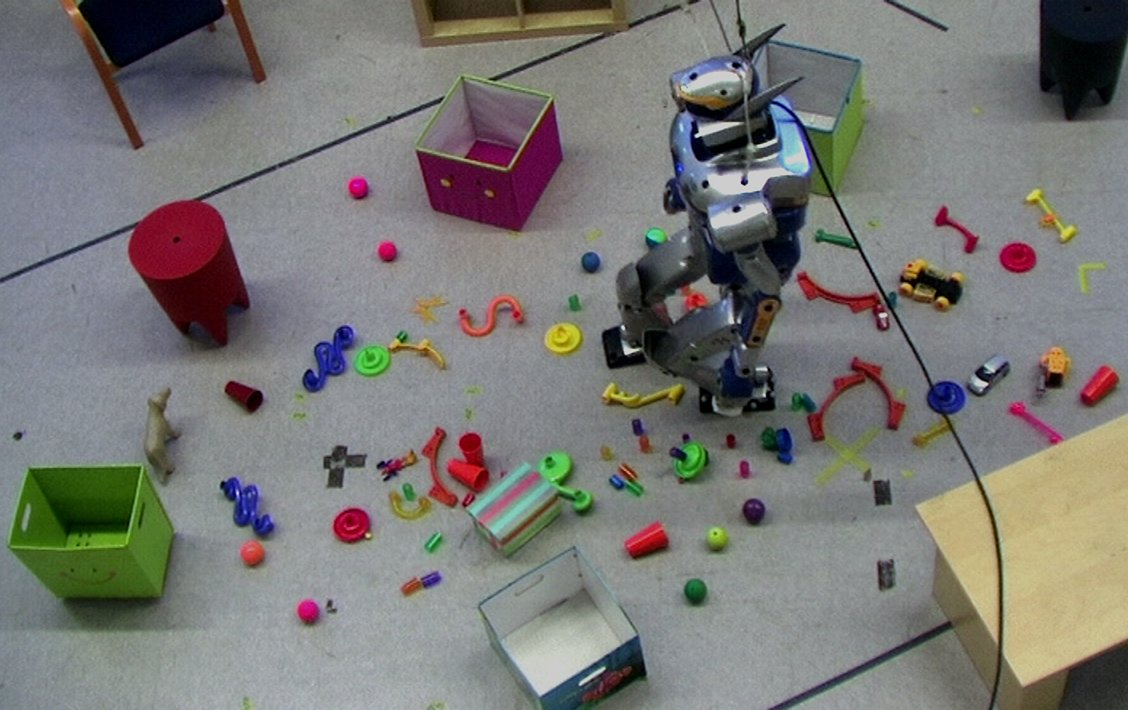
\includegraphics[width=0.45\textwidth]{fig/demo.jpg}
  \end{center}
  \caption{HRP-2 walking in a cluttered environment while avoiding
    obstacles. The final position is reached with a precision of $\pm
    3\mathrm{cm}$. The final error is the consequence of both noise in
    the robot position estimation and drifts in the two last steps
    which happen too late to be not compensated. \label{fig:scenario}}
\end{figure}
%
%
%
Secondly, the new step is validated. The decision is based on the
relative movement of the first corrected foot. Let consider that, for
instance, the next moving foot is the left one. The original left foot
position is \mbox{$s \in \text{SE}(2)$}, the new corrected left foot
position is \mbox{$s' \in \text{SE}(2)$}. The relative position of the
original and new foot is computed. If the $y$ component of the result
is positive, the new step is accepted. In practice, it means that the
step is ``pushed'' away and will not induce an auto-collision. On the
opposite, with the right foot, the step is accepted if the $y$
component is negative.
%
%
If a correction is invalidated, another one is computed during the
next double support phase. In practice, the estimated error during the
next step will be close to the current estimation, in particular the
sign (i.e. direction) of the error will remain the same. As the flying
foot will change the delayed correction has a high probability of
being accepted.
%
%
This naive system has been empirically validated. However, it prevents
some valid corrected steps. In the future, this will be replaced by a
fast on-line steps validation algorithm described by
\cite{10icra.perrin}.
%This algorithm provides fast step validation by
%precomputing feasibility regions offline. This will provide a sound
%and very fast method as the validity checking will be equivalent to
%reading a value in memory.
%
\FloatBarrier
%
%%% Local Variables:
%%% ispell-local-dictionary: "english"
%%% LocalWords:
%%% End:
